\documentclass[12pt]{article}

%%% --- PACKAGES --- %%%
\usepackage{amsmath}
\usepackage{amssymb}
\usepackage{amsthm}
\usepackage{float}
\usepackage{tikz,graphicx,pgfplots}
\usetikzlibrary{patterns,decorations.pathmorphing,positioning}
\pgfplotsset{compat=1.10}
\usepgfplotslibrary{fillbetween}
\usepackage{xcolor}
\usepackage{verbatim}
\usepackage{url}
\usepackage{listings}
\usepackage{enumitem}
\usepackage{booktabs}

%%% --- PAGE LAYOUT --- %%%
\setlength{\textwidth}{168.0truemm}
\setlength{\textheight}{255.0truemm}
\setlength{\oddsidemargin}{-4.0mm}
\setlength{\evensidemargin}{-4.0mm}
\setlength{\topmargin}{-22.0truemm}
\parindent=0mm
\parskip=2mm
\pagestyle{empty}

%%% --- MATH OPERATORS --- %%%
\DeclareMathOperator\artanh{artanh}
\DeclareMathOperator\arsinh{arsinh}
\DeclareMathOperator\arcosh{arcosh}
\DeclareMathOperator\sech{sech}
\newcommand{\ds}{\displaystyle}

%%% --- SOLUTION ENVIRONMENT --- %%%
% Inside the environment: write your solution directly.
% While unanswered, leave the \answerspace{Xcm} command as a placeholder
% (it just reserves vertical space). Delete it once you start writing.
\newenvironment{solution}{%
    \par\vspace{4pt}%
    \noindent\rule{\linewidth}{0.3pt}%
    \par\smallskip%
    \noindent\textit{Solution.}\par\smallskip%
}{%
    \par\noindent\rule{\linewidth}{0.3pt}%
    \par\vspace{6pt}%
}

% Placeholder vertical space — delete this command when writing your solution.
\newcommand{\answerspace}[1][6cm]{\vspace{#1}}

%%% -------------------------------------------------------- %%%
\begin{document}

%%% --- HEADER --- %%%
\begin{center}
    {\bf COLLEGE OF SCIENCE}
\end{center}
\centerline{\large\bf PHYS2020}       % <-- course code
\vspace{0.1cm}
\centerline{\large\bf Simulation Plan}   % <-- assignment number
\vspace{0.1cm}
\centerline{\large\bf Semester One 2026}
\vspace{3mm}
\hrule
\vspace{3mm}

%%% --- STUDENT DETAILS --- %%%
\begin{tabular}{rl}
    & Family name: Lukacs \\[6pt]
    & Given names: Matthew David Carmel\\[6pt]
    & Student number: u8507410\\[6pt]
\end{tabular}

\vspace{4mm}
\hrule
\vspace{4mm}

\subsection{Theory}
\section{Introduction}

When a particle is suspended in a fluid, it undergoes continuous, unpredictable
motion as a result of collisions with the surrounding fluid molecules. This
phenomenon is known as Brownian motion, named after Robert Brown, who documented
it in 1828~\cite{brown1828}. A correct physical explanation was not provided until
Delsaux in 1877~\cite{delsaux1877}, who proposed that the motion arose from
molecular-scale collisions. A quantitative theoretical framework was produced by
Einstein in 1905~\cite{einstein1905}, who derived that the displacement of a
suspended particle along any single axis follows a Gaussian probability
distribution. Perrin subsequently verified this experimentally and was awarded the
Nobel Prize in Physics in 1926~\cite{perrin}. Brownian motion provided some of
the earliest direct evidence for the atomic nature of matter.

This diffusion is linked to statistical and thermal physics.

Einstein showed that the probability distribution function describing the position
of a particle at time $t$ is:
\begin{equation}
    f(x) = \frac{1}{\sqrt{4\pi D t}} \exp\!\left(-\frac{x^2}{4Dt}\right),
    \label{eq:pdf}
\end{equation}
where $D$, the diffusion coefficient, is given by the Stokes-Einstein relation:
\begin{equation}
    D = \frac{k_B T}{6\pi \eta a}.
    \label{eq:stokes}
\end{equation}
Here $T$ is the absolute temperature, $\eta$ is the dynamic viscosity of the
fluid, and $a$ is the particle radius. For two-dimensional motion observed in the
$xy$ plane, the mean squared displacement (MSD) is:
\begin{equation}
    \langle r^2 \rangle = \langle x^2 \rangle + \langle y^2 \rangle = 2Dt + 2Dt = 4Dt,
    \label{eq:msd}
\end{equation}
where the independence of $x$ and $y$ displacements has been
used~\cite{reif1965}. Rearranging Eqs.~(\ref{eq:stokes}) and~(\ref{eq:msd})
gives the working equation:
\begin{equation}
    k_B = \frac{6\pi\eta a D}{T}.
    \label{eq:kB}
\end{equation}
It is also useful to note that Eq.~(\ref{eq:pdf}) takes the Gaussian form:
\begin{equation}
    f(x) = \frac{1}{\sigma \sqrt{2\pi}} \exp\!\left(-\frac{(x - \mu)^2}{2\sigma^2}\right),
    \label{eq:gaussian}
\end{equation}
with $\mu = 0$ and $\sigma^2 = 2Dt$.
based off of my lab report and the phys BM lab manual

\subsection{What I've done so far}
I have now set up a github repository which is also linked to my google drive\\
https://github.com/carmel3141/Brownian-Motion-Simulation-PHYS2020\\
I have tested a few commits to see if i remember how to use github.

yeah so i accidentally bricked my git at one point but its fixed now\\

moved away from the lattice model to a continuous model, which is more realistic and will be more interesting to analyse after reading a couple of websites \\
https://ipython-books.github.io/133-simulating-a-brownian-motion/ \\
https://www.quantstart.com/articles/brownian-motion-simulation-with-python/ \\

one of these has a continuous one where it uses a polar co-ordinate system to generate the random walk which would be interesting to try too\\

\section{What im currently working on}
currently reading :\\
https://matplotlib.org/stable/users/explain/animations/animations.html\\
to hopefully make this a live simulation, will also plug in some actual physics constants and base the walk off of my theory, and introduce multiple particles.



\begin{center}
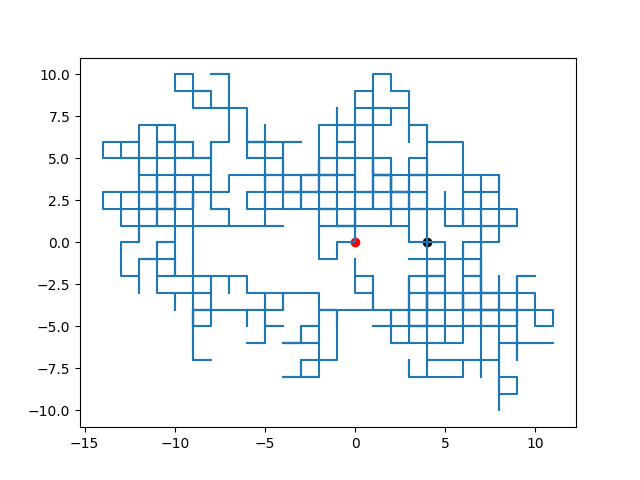
\includegraphics[width=0.8\textwidth]{trial1.png}
\end{center}
trial 1. added start point and end point, current version has legend too

\begin{center}
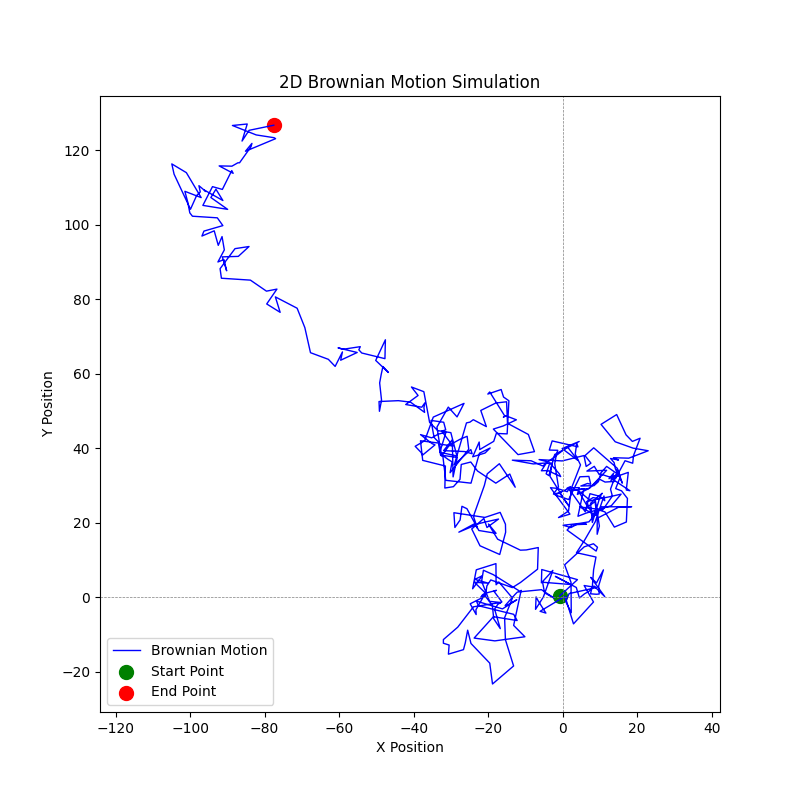
\includegraphics[width=0.8\textwidth]{trial_2.png}
\end{center}
now uses interpolation instead of grid/lattice so it's more continuous with time-steps, much better !!! 

\begin{center}
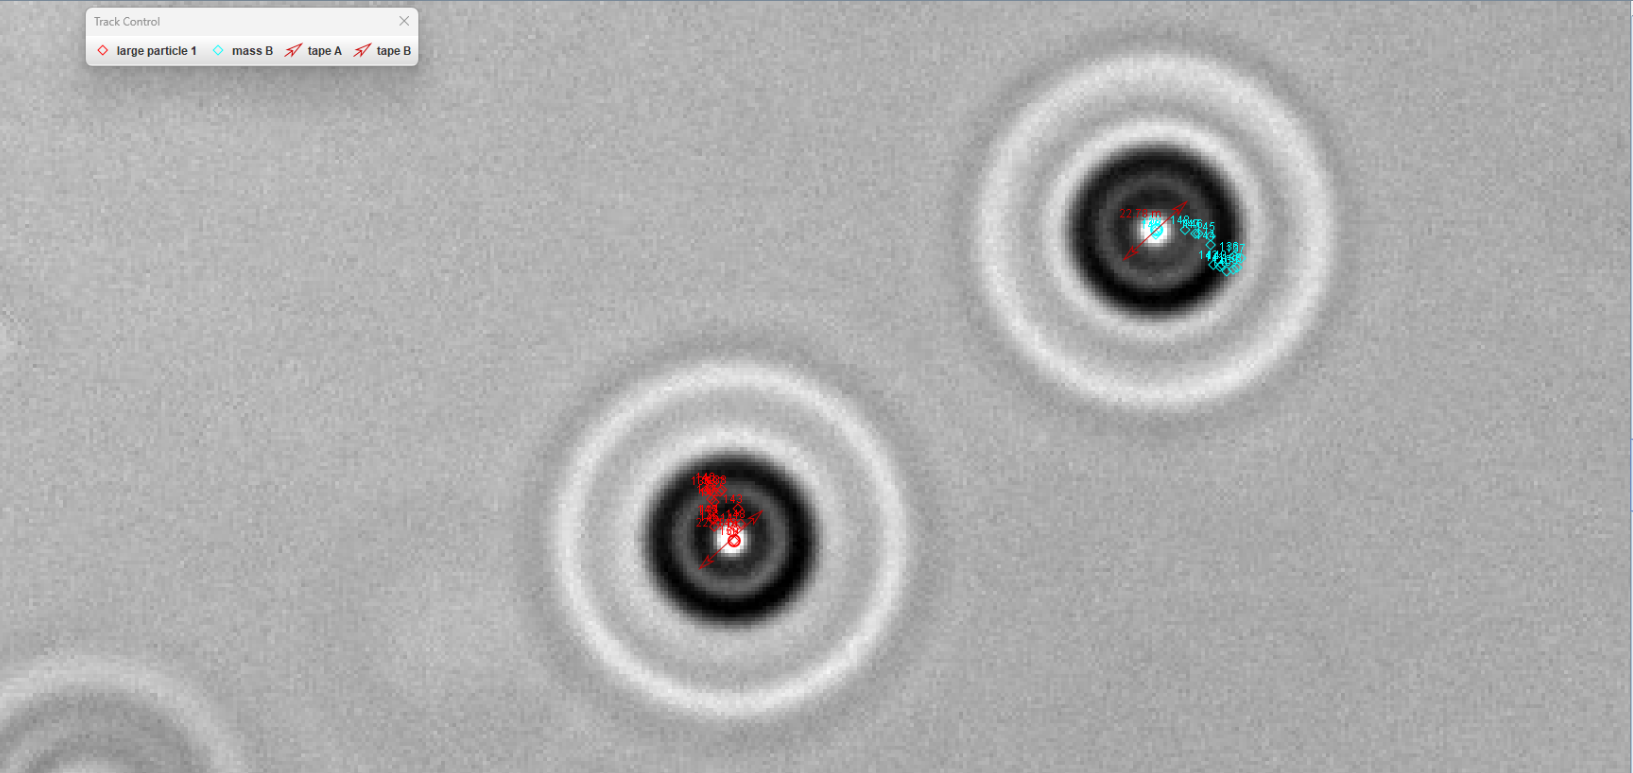
\includegraphics[width=0.8\textwidth]{large trk 1 particle a and B.png}
\end{center}
a real photo taken by myself and a lab parter of particles exhibiting brownian motion



\newpage
\begin{thebibliography}{99}

\bibitem{brown1828}
R.~Brown,
“A brief account of microscopical observations on the particles contained in the pollen of plants and the general existence of active molecules in organic and inorganic bodies,”
\textit{Edinburgh New Philosophical Journal}, p.~358 (1828).

\bibitem{delsaux1877}
J.~Delsaux,
(1877).

\bibitem{einstein1905}
A.~Einstein,
“Über die von der molekularkinetischen Theorie der Wärme geforderte Bewegung von in ruhenden Flüssigkeiten suspendierten Teilchen,”
\textit{Annalen der Physik (Leipzig)} \textbf{17}, 549 (1905).
English translation: \textit{Investigations on the Theory of the Brownian Movement}, Dover (1956).

\bibitem{perrin}
J.~Perrin,
“Le mouvement Brownien et la réalité moléculaire,”
\textit{Annales de Chimie et de Physique} \textbf{18}, 5 (1909).
English translation: \textit{Brownian Movement and Molecular Reality}, translated by F. Soddy, Taylor \& Francis (1910).

\bibitem{reif1965}
F.~Reif,
\textit{Fundamentals of Statistical and Thermal Physics},
McGraw-Hill, New York (1965), Chapter 15.

\bibitem{tracker}
Tracker Video Analysis and Modeling Tool,
\url{https://physlets.org/tracker/} (accessed 2026).

\bibitem{labmanual}
PHYSICS ANU Laboratory Manual, Brownian Motion
Australian National University (2026).

\bibitem{viscosity}
Water viscosity data table,
\url{https://chem-casts.com/data-tables/water-viscosity-data-table} (accessed 2026).

\bibitem{boltzmann}
National Institute of Standards and Technology (NIST),
\url{https://physics.nist.gov/cgi-bin/cuu/Value?k} (accessed 2026).

note: origin of the references are mostly from the lab manual and some are here for future reference


\end{thebibliography}













\end{document}